\documentclass[12pt]{article}
\usepackage{graphics, verbatim, multicol}
\usepackage{color}
\usepackage{listings}

\definecolor{gray}{rgb}{.4,.4,.4}

\newcommand{\titleize}[1]{
   \begin{center}
       \Large \textsc{#1} \normalsize \\
   \end{center}
}

\newcommand{\normaltitleize}[1]{\mbox{}\\ \textsc{#1} \normalsize}

\newcommand{\headerstuff}{
   \begin{center}
   \textsc{\Large{Alpheus Madsen}}

   \rule{1in}{.01in}

   961 South 200 East \\

   Orem, UT \ \ 84058  \\

   (435)363-5968 \\

   alpheus.madsen@gmail.com

   \rule{2in}{.01in}
   \end{center}
}

\newcommand{\sectionline}{
\begin{center}
   \rule{1in}{.01in}
\end{center}
}

\title{A Simple 3D Graphics Engine}
\author{\headerstuff}
\date{}

\begin{document}
\lstset{language=Python, basicstyle=\ttfamily\color{blue}, keywordstyle=\bf\color{blue}, stringstyle=\color{red}, commentstyle=\em\color{gray},
showstringspaces=false,
identifierstyle=\color{black},
numbers=none, numberstyle=\tiny\color{gray}}

%\maketitle
\headerstuff

\titleize{A Simple 3D Graphics Engine\\Written in Python and Allegro}

\normaltitleize{Introduction.}  This is the source code of a program I wrote during my first summer as a graduate student.  My program implements a 3D camera, draws a coordinate axis for reference, and then draws eight cubes being rotated around different rotational axes.  (The rotations are implemented through a combination of quaternion multiplication and quaternion-to-matrix conversion.)  In addition to rotating the cubes individually, the entire system is rotated around the $x$-axis.  By pressing any key, the rotational axis is switched to the $z$-axis, then the $y$-axis, and finally the unit vector in the direction of the vector $(5, 5, 2)$; another press then ``freezes'' the system (while the cubes continue to rotate), and a final press then causes the camera to ``ride away'' from the system.  (Figure~\ref{screenshots} shows some screen shots.)

\begin{figure}[!hbtp]
   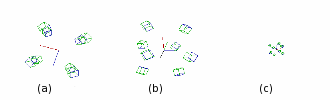
\includegraphics{screenshots4.png}
\caption{Three screen shots from ``littlecubesystem.py'': (a) rotation of system around the $z$-axis, (b) rotation of system around the vector $(5, 5, 2)$, and (c) camera ``rides away'' from the system.}\label{screenshots}
\end{figure}

The source code of this program is split into several files; each file is prefaced with a brief introduction.

\normaltitleize{Dependencies.}  This program relies specifically on \emph{Allegro~4.2.2} and \emph{Alpy~0.1.3} (it doesn't seem to work with later versions), and Python~2.2 or greater.  It should also be noted that I have only attempted to use this program under Linux; I have no idea how well it would run under other operating systems.

Allegro is a game, graphics and sound library that can be downloaded from ``http://alleg.sourceforge.net''.  Several years ago a friend introduced me to this library, and I like this library enough that I wanted to use it for this project.  In particular, Allegro provides a system for doing graphics independent of the X Window system; since I had a desire (and still do, actually) to put together an ``open source'' game console, creating a game that didn't use the overhead of the X Window system was very appealing.

Alpy is a package that provides bindings that I needed to use Allegro under Python.  Although these bindings don't provide complete Allegro functionality, they provide enough for me to work on this project.  This package can be downloaded at ``http://pyallegro.sourceforge.net/alpy.php'', but because the newer version of Alpy doesn't seem to work, it is necessary to download an older version.  To do so,
\begin{enumerate}
   \item Scroll down to the section ``Alpy 0.1.3 released'',

   \item and click on the link ``SourceForge's file section'',

   \item Scroll down and select ``alpy-0.1.3'', and then decide which version (.tar.gz or .zip) to download.
\end{enumerate}

This package also requires Python 2.2 or greater.  I chose to write this program in Python because Python is a powerful yet easy-to-learn scripting language that can be mixed relatively easily with C or C++.  These features make Python ideal as a prototyping language.

\normaltitleize{Future Goals for This Project.}  Having completed my camera apparatus, I had hoped to make a wireframe chess piece, and then expand my 3D engine to include the following:
\begin{itemize}
   \item Filling in of faces, and establishing appropriate drawing orders;

   \item Clipping and ``distance fog'', to limit the number of polygons needed to write to the screen;

   \item A physics engine, to realistically represent momentum, inertia, gravity, rotational momentum, and so forth;

   \item Ability to move characters using a keyboard or joystick.

   \item Re-implementation of the classes to make objects easier to manipulate;

   \item Re-implementation of crucial portions in C++, to increase the speed of the program.
\end{itemize}
In particular, I hope to expand this engine to become a computer game.  My goals in this regard were delayed as my graduate studies intensified.

\normaltitleize{Personal Remarks.}  Since high school I have always been interested in programming computer games.  It is a little unfortunate that my interest began in a time when 3D game engines were coming of age; my career wouldn't be able to mature with the industry.  I couldn't start my career with a simple yet popular game like Pong (that, despite its simplicity, taxed the available computing resources at the time) and continue writing more complex programs, eventually leading up to a game like Doom III.  Instead, I have the desire (and the far more difficult goal) to write a full-fledged 3D computer game!

Even so, I have always had an affinity with writing 3D programs; this field fuses together computer programming with linear algebra in a concrete, visual way.  Due to my studies as a graduate student, however, and the complexities of such a project, I simply have not had the time to pursue this project as much as I would have liked.

%\newpage
\sectionline

\normaltitleize{``math3d.py''.}  This module conveniently brings together all the modules I wrote for my 3D graphics engine.  It's rather boring!  I decided to put it first, as a sort-of table of contents of the rest of the modules.

\lstinputlisting{math3d.py}

% \newpage

\sectionline

\normaltitleize{``ttable.py''.} In this module, I define special trigonometric functions that rely on table lookups rather than direct computation; I use ``bradians'' as an alternative to radians or degrees to take advantage of the binary nature of computers:  one byte will contain all possible bradian values.

\lstinputlisting{ttable.py}

%\newpage

\sectionline

\normaltitleize{``vertex.py''.} This module contains everything convenient for working with vertices (represented as vectors), edges and faces.  I first define the vector class and vector algebra, then go on to define edges and faces, and end by defining two useful ``palettes'' of colors.

\lstinputlisting{vertex.py}

% \newpage

\sectionline

\normaltitleize{``matrix.py''.}  This next module defines some matrix algebra, and produces various matrices (including camera matrices) that would be useful in working with computer graphics.

\lstinputlisting{matrix.py}

% \newpage

\sectionline

\normaltitleize{``movable.py''}  This module creates the class that is the foundation for all my 3D objects.

\lstinputlisting{movable.py}

% \newpage

\sectionline

\normaltitleize{``wf.py''.}  This module provides the class that reads in data files and uses them to create wireframe objects.

\lstinputlisting{wf.py}

% \newpage

\sectionline

\normaltitleize{``camera.py''.} This next module defines two different cameras that could be used to render a scene.  This is the core of the 3D graphics engine.

\lstinputlisting{camera.py}

% \newpage

\sectionline

\normaltitleize{``littlecubesystem.py''.}  This file uses my camera, as implemented in the previous modules, and displays the rotating cubes.

\lstinputlisting{littlecubesystem.py}

% \newpage

\sectionline

\normaltitleize{The data file ``littlecube.dat''.}  This contains the information needed to create a cube.  The comments in this file also explain how to write (or generate via software) other wireframe files.

\verbatiminput{littlecube.dat}

% \newpage

\sectionline

\normaltitleize{The data file ``coords.dat''.}  This data file provides the coordinate axis that is drawn by the program.

\verbatiminput{coords.dat}

% \newpage

\sectionline

\normaltitleize{``sintable.dat''.}  For completeness, the data for the bradian sine table is also provided, although this file is just a list of computer-generated numbers.  It starts with the bradian sine of $0$, and then increments up to the bradian sine of $255$.

In the original text file, these numbers are in a single column; to save space (and to make it more readable), these numbers are shown here in three columns.

\begin{multicols}{3}
\verbatiminput{sintable.dat}
\end{multicols}

\end{document}
